%%%%%%%%%%%%%%%%%%%%%%% file template.tex %%%%%%%%%%%%%%%%%%%%%%%%%
%
% This is a general template file for the LaTeX package SVJour3
% for Springer journals.          Springer Heidelberg 2006/03/15
%
% Copy it to a new file with a new name and use it as the basis
% for your article. Delete % signs as needed.
%
% This template includes a few options for different layouts and
% content for various journals. Please consult a previous issue of
% your journal as needed.
%
%%%%%%%%%%%%%%%%%%%%%%%%%%%%%%%%%%%%%%%%%%%%%%%%%%%%%%%%%%%%%%%%%%%
%
% First comes an example EPS file -- just ignore it and
% proceed on the \documentclass line
% your LaTeX will extract the file if required
\begin{filecontents*}{example.eps}
%!PS-Adobe-3.0 EPSF-3.0
%%BoundingBox: 19 19 221 221
%%CreationDate: Mon Sep 29 1997
%%Creator: programmed by hand (JK)
%%EndComments
gsave
newpath
  20 20 moveto
  20 220 lineto
  220 220 lineto
  220 20 lineto
closepath
2 setlinewidth
gsave
  .4 setgray fill
grestore
stroke
grestore
\end{filecontents*}
%
\documentclass{svjour3}                     % onecolumn (standard format)
%\documentclass[smallextended]{svjour3}     % onecolumn (second format)
%\documentclass[twocolumn]{svjour3}         % twocolumn
%
\smartqed  % flush right qed marks, e.g. at end of proof
%
\usepackage{graphicx}
%
% \usepackage{mathptmx}      % use Times fonts if available on your TeX system
%
% insert here the call for the packages your document requires
%\usepackage{latexsym}
% etc.
%
% please place your own definitions here and don't use \def but
% \newcommand{}{}
%
% Insert the name of "your journal" with
\journalname{JournalofGridComputing}
%
\begin{document}

\title{Distributed Analysis in CMS}
%\subtitle{Do you have a subtitle?\\ If so, write it here}

\author{Alessandra Fanfani \and Akram Kahn \and Andrea Sartirana \and Aresh Vedaee \and Andrea Sciab\`a \and Anzar Afaq \and Barry J. Blumenfeld \and Bockjoo Kim \and Carlos Kavka \and Chih-Hao Huang \and Chris Brew \and Christoph Wissing \and Claudio Grandi \and Daniele Bonacorsi \and Daniele Spiga \and Daniel Riley \and Dave Evans \and David Dykstra \and Derek Feichtinger \and Edward Karavakis \and Eric Vaandering \and Eric Wicklund \and Fabio Farina \and Federica Fanzago \and Frank W\"urthwein \and Gerhild Maier \and Giuseppe Codispoti \and Giusepppe Bagliesi \and Haifeng Pi \and Hassen Riahi \and Ian Fisk \and Ilaria Villella \and Kati Lassila-Perini \and Kejing Kang \and Ken Bloom \and Lassi Tuura \and Lee Lueking \and Liang Dong \and Lothar Bauerdick \and James Letts \and Jorgen D'Hondt \and Joris Maes \and Jose Afonso Sanches \and Jose' M. Hern\`andez \and Josep Flix \and Jukka Klem \and Julia Andreeva \and Marco Calloni \and Mattia Cinquilli \and Nicolo' Magini \and Pablo Saiz \and Patricia Bittencourt Sampaio \and Paul Rossman \and Peter Elmer \and Peter Kreuzer \and Petra Van Mulders \and Ricky Egeland \and Sanjay Padhi \and Simon Metson  \and Stefano Belforte \and Stefano Lacaprara \and Thomas Kress \and Tibor Kurca \and Tony Wildish \and Valentin Kuznetsov \and Vijay Sekhri \and Vincenzo Miccio \and Yuyi Guo }

\authorrunning{} % if too long for running head

\institute{A. Fanfani \and D. Bonacorsi \and G. Codispoti \and C. Grandi
           \at INFN and University of Bologna, viale Berti Pichat 6/2, 40127 Bologna, Italy \\
              Tel.: +39-51-2095232 Fax: +39-51-209XXXX\\
              \email{fanfani@bo.infn.it}
%             \emph{Present address:} of F. Author  %  if needed
           \and
           G. Donvito \at INFN and University of Bari
           \and
           S. Metson \at Bristol University, UK
           \and
           E.Karavaki \and A.Khan \at Brunel University, UK
           \and
           J. D'Hondt \and J.Maes \and P. Van Mulders \and I. Villella \at Brussel University, Belgium
           \and 
            M. Calloni \and D. Spiga \and A.Sciab\`a \and J. Andreeva \and P. Saiz \at CERN, Switzerland
           \and
           N. Magini \and V. Miccio \at CERN, Switzerland and INFN-CNAF, Italy 
           \and
            J. M. Hern\`andez \at CIEMAT, Madrid, Spain
           \and
            J. Flix \at CIEMAT, Madrid, Spain  and PIC, Barcelona, Spain
           \and
            D. Cesini \and D. Dongiovanni \at INFN-CNAF, Italy
            \and
            L. Dong \at Institute of High Energy Physics, Chinese Academy of Sciences Academia Sinica, Cina
           \and
           V. Kuznetsov \and D. Riley \at Cornell University, Ithaca, NY, USA
           \and
           Ch. Wissing \at DESY,  Germany
           \and
           A. Afaq \and L. Bauerdick \and D. Dykstra \and D. Evans \and I. Fisk \and Y. Guo \and C. Huang \and L. Lueking \and P.Rossman \and V. Sekhri \and E.Vaandering \and E.Wicklund \at Fermilab, Batavia, IL, USA
           \and
           B. Kim \at University of Florida, Gainesville, FL, USA
           \and
           J. Klem \and K. Lassila-Perini \at Helsinki Institute of Physics, Finland
           \and
           S. Lacaprara \at Legnaro INFN, Italy
           \and 
           G.Maier \at University of Linz, Austria
           \and
           T. Kurca \at Institut de Physique Nucleaire de Lyon, France
           \and
           F. Farina \at Milano Bicocca INFN, Italy
           \and
           R. Egeland \at University of Minnesota, Twin Cities, MN, USA
           \and
           K. Bloom \at University of Nebraska, NE, USA
           \and
           L. Tuura \at University of Northeastern, Boston, MA, USA
           \and
           B.Blumenfeld \at Johns Hopkins University, Baltimore, MD, USA
           \and
           F. Fanzago \at Padova INFN, Italy
           \and
            K. Kang \at Peking University, Cina
           \and
           M. Cinquilli \and H. Riahi \and A. Vedaee \at Perugia INFN, Italy
           \and
           G. Bagliesi \at Pisa INFN, Italy
           \and
           A. Sartirana \at Ecole Polytechnique, Paris, France
           \and
           P. Elmer \and T. Wildish \at Princeton University, Princeton, NJ, USA
           \and
           D. Feichtinger \at Paul Scherrer Institut (PSI), Switzerland
           \and
           C. Brew \at Rutherford Appleton Laboratory, UK
           \and
           T. Kress \and P. Kreuzer \at RWTH , Germany
           \and
            P. Bittencourt Sampaio \and J. Afonso Sanches \at University of Rio De Janeiro UERJ, Brasil
           \and
           J. Letts \and S. Padhi \and H. Pi \and F. W\"urthwein \at University of California San Diego, LaJolla, CA, USA
           \and
           S. Belforte \and C. Kavka \at Trieste INFN, Italy
}

\date{Received: date / Accepted: date}
% The correct dates will be entered by the editor


\maketitle

\begin{abstract}
CMS expects to manage several Pbytes of data each year, distributing them
over many computing sites around the world and enabling data access at those
centers for analysis. CMS has identified the distributed sites as the primary
location for physics analysis to support a wide community of users,
potentially as many as 3000 users. This represents an unprecedent scale of
distributed computing resources and number of users.
An overview of the computing architecture, the software tools and
the distributed infrastructure deployed is reported.
Summaries of the experience in establishing efficient and scalable operations
to prepare for CMS distributed analysis are presented, followed by
the user experience in their current analysis activities.
\keywords{LHC \and CMS \and Distributed Analysis}
% \PACS{PACS code1 \and PACS code2 \and more}
% \subclass{MSC code1 \and MSC code2 \and more}
\end{abstract}

\section{Introduction}
\label{intro}
The Compact Muon Solenoid (CMS) ~\cite{RefCMS} is a general-purpose detector
that will collect data at the Large Hadron Collider (LHC),located at CERN
(Geneva).
%The Compact Muon Solenoid (CMS) detector~\cite{RefCMS} is a general-purpose detector
%designed to exploit the physics potential at the Large Hadron Collider (LHC),
%located at CERN (Geneva).
The beams will collide at the rate of 25 ns and CMS will record only the collisions
that pass a set of %real time 
online trigger decisions with an expected rate around 300Hz and an
average event size of 1-2 MB. A nominal year worth of data taking 
corresponds to about 2-6 PB of storage prior to any processing.
Data will have to be accessed for reprocessing and analysis by a
large experimental community with more than 3000 collaborators distributed
worldwide across 40 countries. This imposes an unprecedented computing
challenge for data management and processing.

%\paragraph{Paragraph headings} Use paragraph headings as needed.
\section{The CMS Computing Model}
\label{sec:2}
The CMS distributed computing and analysis model ~\cite{RefCM} is designed to serve, process and archive the %huge amount of data the experiment will collect.
%large amounts of events that will be available when the detector starts collecting data.
large number of events that will be generated when the CMS detector starts taking data. The computing resources are geographically distributed, interconnected via high throughput networks and accessed via by means of Grid software. 
%%  motivations to choose a distributed environment
The choice of a distributed system allows to delegate responsibilities to local CMS communities, access to additional funding channels and ensure load balancing of the available resources while replicating the interesting data in different sites.


A multi-Tier hierarchical distributed model is adopted in CMS with specific functionality at different levels.
%\subsection{Tier-0}
%\label{sec:2_1}
\paragraph{Tier-0:}
The Tier-0 centre at CERN accepts data from the CMS online system, archives the data, performs prompt first pass reconstruction. Reconstructed data at the Tier-0 together with the corresponding raw data are distributed to Tier-1s over the Optical Private Network that is the backbone network specifically built for LHC to interconnect CERN and the Tier-1s.
In addition to the Tier-0 centre, CERN hosts the CMS Analysis Facility (CAF) that is focused on latency-critical detector, trigger and calibration activities.
Roughly 20\% of the computing capacity is located at CERN, while the remaining is distributed.

%\subsection{Tier-1}
%\label{sec:2_2}
\paragraph{Tier-1:} 
Each Tier-1 centre assures the distributed custodial storage of a fraction of the raw data produced by the CMS detector and for the simulated data produced at the connected Tier-2 centres; provides computing resources for their further re-processing (re-reconstruction, skimming, etc…) and for high priority analysis; controls the data transfer to the Tier-2 centres for analysis. There are 7 Tier-1 centres located in France, Germany, Italy, Spain, Taiwan, United Kingdom and United States.

%The Tier-1 are 7 large regional computing centers located in France, Germany, Italy, Spain, Taiwan, United Kingdom and United States, where organized mass data processing are performed. That includes re-processing, data skimming and other organized intensive analysis tasks. 
%%From CM CHEP09: For reconstruction a nominal Tier-1 should be capable of processing 70Hz worth of data with a required IO rate of 100MB/s. Skimming through the reconstructed datasets uses only 1\% of CPU of reconstruction so sparse reading of the file is required to have manageable IO rates.
%The Tier-1 centres archive the fraction of data distributed to them as well as the simulated data produced at the Tier-2 centres,  while they are serving analysis transfer requests to Tier-2.
%%From CM CHEP09: In the CMS experiment the Tier-1 centers rather than the Tier-0 serve the majority of the data to the Tier-2 centers for analysis.

%\subsection{Tier-2}
%\label{sec:2_3}
\paragraph{Tier-2:}
Tier-2 centers, more than 50 sites around the world,  provide capacity for user data analysis and for production of simulated data.
In CMS data transfer to Tier-2 can occur from any Tier-1. A significant effort is required in 
commissioning all possible transfer links, as described in section ~\ref{sec:LinkCommissioning}, as well
as improving site availability, as described in section ~\ref{sec:4_2_1}.

\section{Framework for CMS Distributed Analysis}
\label{sec:3}
The CMS analysis model foresees activites driven by data location. Data are distributed over many computing centers according to CMS data placement policies. Processing takes place where data are located. In order to enable distributed analysis a set of Workload and Data Management tools have been developed, building CMS-specific services on top of existing Grid services.

\subsection{Data Management}
\label{sec:3_1}
The CMS Data Management System provides the basic infrastructure and tools necessary to manage the large amounts of data produced, processed and analysed in a distributed computing environment. 
In order to simplify bulk data management, files are grouped together into “file-blocks”  of a convenient size for data transfer. %the exact choice of the size of the file blocks will depend on the type of data. 
File-blocks are in turn grouped in datasets whose size is driven by physics.
The file-block is the unit of data location and replication. 
The tracking of data location is file-block based and it provides the name of sites hosting the data, not the physical location of constituent files at the sites nor the composition of file-blocks.
The file-block contains files that can be processed and analyzed together.
%Processing is block-based. 
The packaging of events into files is done so that the average file size is
kept reasonably large (e.g. at least 1GB), in order to avoid scaling issues with storage and tape systems and to optimize data transfer.
This is achieved merging small outputs files produced by individual jobs in fewer larger files.

The CMS Data Management System is made of a set of loosely coupled components as described in the following sections.
\subsubsection{DBS}
\label{sec:3_1_1}
The Dataset Bookkeeping Service (DBS)\cite{RefDBS} provides the means to describe, discover and use CMS event data. 
It catalogs CMS specific data definitions such as run number, the algorithms and configurations used to process the data together with the information regarding the processing parentage of the data it describes.
The DBS stores information about CMS data in a queryable format. The supported queries allow to discover available data and how they are organized logically in term of packaging units like files and file-blocks. The information available from queries to DBS are site independent.

The DBS is used for data discovery and job configuration by the production and analysis systems through a DBS API. 
Users can discover what data exists using a Web browser or Command Line Interface.
The DBS is usable in multiple “scopes”:
\begin{itemize}
\item A Global scope DBS is a single instance describing data CMS-wide %all data used by the experiment
\item Many local scopes are established to describe data produced by MonteCarlo production, Physics groups or individuals. %Data described in local scope will eventually be migrated to the global scope. 
Data produced in local scope may be migrated to global scope as needed.

\end{itemize}
The DBS system is a multi-tier web application whose design is modular and makes it easily adaptable to multiple database technologies. The supported types of database (ORACLE, MySQL and SQLite) enable the DBS deployment in a range of environments from general CMS at large installations to specific personal installations.
An XML format is used for the format of the HTTP payload exchanged with the client.

The Global DBS is hosted at CERN and its database engine is the CERN Oracle RAC (Real Application Cluster) server for CMS. Some local scope DBS instances that catalog data from Physics groups are also hosted at CERN. There are also DBS instances installed at other sites for private use. 
% If possible find out the amount of data (datasets,files) described so far in Global DBS

\subsubsection{Local Data Catalogue}
\label{sec:3_1_2}
A CMS application only knows about logical files and relies on a local catalogue service to have access to the physical files.
Each CMS site has a Trivial File Catalogue made of simple rules to build site-specific physical paths starting from logical file names and access protocols.
%Local file catalogues provides site local information about how to access any given logical file name. This file catalogue returns the physical location of a logical file within the site itself. 

\subsubsection{Conditions Data}
\label{sec:3_1_3}
%% CR-2009/073 
The data describing the alignment and calibration of the detector are known as ''conditions data''. Since the same conditions data need to be accessed by many processing jobs worldwide CMS uses a caching system called Frontier~\cite{RefFrontier}.
Frontier translates database queries into HTTP, looks up the results in a central database at CERN, and caches the results in an industry-standard HTTP proxy/caching server called Squid. Squid servers are deployed at each site. Conditions data is read by the applications from these Squid servers.

\subsubsection{PhEDEx}
\label{sec:3_1_4}
The CMS data placement and transfer systems are implemented by
PhEDEx\cite{RefPhEDEx}. The data placement system provides an
interface to define, execute and monitor administrative decision of
data movement such as where experiment data is to be located, which
copies are custodial, and %to which physics analysis group the data is allocated for.  
the physics analysis group a given set of data is replicated for at a given site.
Data are distributed according to available resources
and physics interests at sites as determined by CMS Data Operations,
physics analysis groups, and/or the members of the "local" CMS community the site serves. 
%and/or the site data managers.

In PhEDEx, distinct storage areas (grid sites or disk/tape areas
within a site) are represented by a node.  Links between the nodes
define the transfer topology.  The transfer workflow begins when a
user makes a transfer request of some data to some node via the web
page, which is then approved by that node's Data Manager.  In the
request, the user only specifies the destination node, and the optimal
source node is determined from among the available file replicas.  To
do this, PhEDEx uses Dijkstra's algorithm to calculate the path of
least cost, where cost of transfer for each link is determined by the
recent transfer rate and the size of the current queue over that link.
Using this method, PhEDEx balances exports among multiple sources when
the same data is requested to multiple nodes, and is also
fault-tolerant when links fail to perform and another source replica
is available.

Technically PhEDEx is based on software agents storing their state and
communicating via a central ``black board'' database hosted in the
CERN Oracle RAC (Real Application Clusters). A set of service agents
run centrally at CERN while each site in general runs
only the agents that interact with the storage at the site. The usual
method of transfer execution is to submit a job to File Transfer System (FTS), 
which is managed by the site download agent using the FTS backend.  Download
agent backends for other transfer methods are available, making PhEDEx
technology independent. A web site offers various management tools,
including the request creation and approval interfaces, and allows
users and site administrators to monitor current and historical
transfer conditions.  File deletion and on-demand consistency checking
are also provided by agents running at the site receiving work queues
from the central database.  A web data service provides
machine-readable XML or JSON data from the database, which is used to
integrate PhEDEx with other CMS computing components.  For instance,
PhEDEx keeps track of data location in the distributed computing
system and the analysis system relies on the data service to obtain
the locations of the data when submitting jobs.

\begin{figure}
 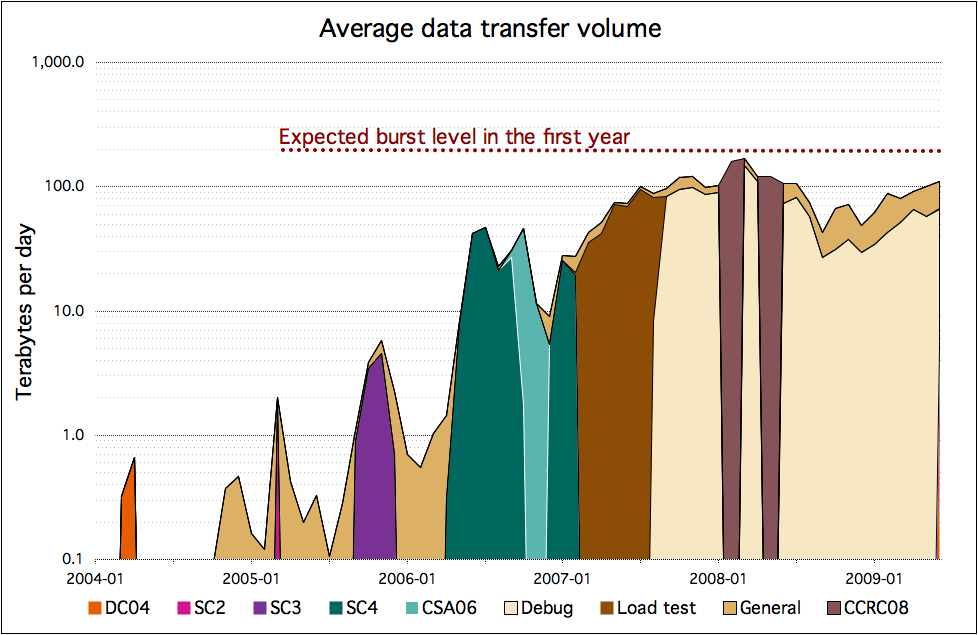
\includegraphics[width=0.70\textwidth]{figures/phedex-avg-monthly-volume.png}
\caption{Average daily transfer volume per month using PhEDEx since the project began.}
\label{fig:phedex-transfers}
\end{figure}

Using PhEDEx, CMS has transferred over 87 PB of data since the project
begain in 2004.  Figure \ref{fig:phedex-transfers} shows the average
daily transfer volume per month of data managed by PhEDEx from
mid-2004 until July 2009.  Varios challenge periods are highlighted,
and in particular the SC4, CSA06~\cite{RefPastExp}, and LoadTest/Debug periods resulted
in large increases in average transfer volume.  ``General'' transfers
include transferring of Monte Carlo or cosmics raw data for physics
analysis.  ``Debug'' and ``LoadTest'' transfers are of randomly
generated data for the purpose of debugging and commissioning the
transfer fabric.  In the first 6 months of 2009 PhEDEx has maintained
average daily transfer volumes of over 80 TB per day, where roughly
40\% of the traffic has been ``General'' production/analysis traffic
and the remaining 60\% ``Debug'' commissioning traffic.  Expected
burst levels during LHC data taking are at 200 TB per day, and such
levels have already been demonstrated by PhEDEx in late February 2008
during the Common Computing Readiness Challenge (CCRC08) challenge.

\subsection{Workload Management}
The role of the CMS Workload Management system includes the interpretation of user processing requests, the creation of the jobs that process the data, the submission of the jobs to local or distributed systems, the monitoring of the jobs and the retrieval of their outputs. The Production Agent (ProdAgent)\cite{RefPA} is a tool optimized to perform these operations in a controlled environment i.e. at the Tier-0 and at the Tier-1 centres. The CMS Remote Analysis Builder (CRAB) is optimized for user analysis.

%
\label{sec:3_2}
\subsubsection{CRAB}
\label{sec:CRAB}
The CMS Remote Analysis Builder (CRAB)\cite{RefCRAB} has been developed as a user-friendly interface to handle data analysis in a local or distributed environment, hiding the complexity of interactions with the Grid and CMS services.
It allows the user to run over large distributed data samples with the same analysis code he has developed 
locally in a small scale test. 

The functionalities that CRAB provides, as schematically illustrated in Fig.~\ref{fig:CRABWorkflow}, are:
\begin{itemize}
\item{Data discovery and location:}
Facilitate queries of the experiment data catalogues (DBS and PhEDEx) to find which data and where it is to be accessed.
\item{Job preparation:}
Pack local user code and the environment to be sent to remote sites where the CMS software is pre-installed as described in ~\ref{sec:4_1_3}.
\item{Job splitting:}
Decide how to configure each job to access a subset of files in the dataset to effectively use the Tier-2s resources.
\item{Job submission:}
Submit to Grid sites hosting the user required data.
\item{Job monitoring:}
Monitor the status of the submitted jobs querying Grid services.
\item{Handling Output data:}
Copy the produced output to a remote Tier-2 the user is associated with or return it to the user for small files (few MB).
Publish the produced data with their description and provenance into a local DBS so that the data can be used in further analysis and shared with other colleagues.
\end{itemize} 

%% Grid integration via BOSSLite
CRAB is coded in Python. The interface to the Grid middlewares and local batch systems is provided by a Python library named BOSSLite\cite{RefBOSSLite}. It relies on a database to track and log information about the user requested task into an entity-relation schema.
An abstract interface is used to access the database through safe sessions and connection pools to grant safe operation in a multiprocessing/multi threaded environment. The current implementation supports MySQL and SQLite databases.
Standard operations such as job submission, tracking, cancellation and output retrieval are also performed via a generic abstract interface. Scheduler (batch system or grid) specific interfaces are implemented in plug-ins, loaded at run-time. Presently, plug-ins are implemented for the Grid middleware EGEE (gLite) \cite{RefgLiteWMS}, OSG \cite{RefOSG} both direct Condor-G submission or a pilot based job submission system(glideinWMS\cite{Refglidein}), and ARC (NorduGrid)\cite{RefARC}.In addition plug-ins for batch systems such as LSF and SGE are provided.
%\emph{FIXME: are few lines about grid specific implementation required? Such as the following lines about gLite}
%Using the gLite WMS BOSSLite enables bulk job submission through gLite collections. This allows a faster job submission, but also an optimized job status tracking through bulk queries. Since the CMS computing model uses its own data location system, the gLite WMS match making has the main role to perform a load balancing among sites that are hosting the data to be accessed. 

%% CRAB server motivation and architecture:
The interaction with the Grid can be either direct with a thin CRAB client or using an intermediate CRAB Analysis Server~\cite{RefCRAB} (see Fig.~\ref{fig:CRABWorkflow}). The CRAB Analysis Server automates the user analysis workflow with resubmissions, error handling, output retrieval thus leaving to the user just the preparation of the configuration file and notifying him of the output availability. In addition it has the capability of implementing advanced analysis use cases.
The Analysis Server is made of a set of independent components communicating asynchronously through a shared messaging service and cooperating to carry out the analysis workflow. The communication between client and server is implemented using the gSOAP framework and Grid credentials of users are delegated to server.
The Analysis Server is coupled with an external GridFTP server %Storage Element
 that stores the user input and output data, allowing to implement CMS policies on sandbox sizes, bypassing for instance the gLite WMS limits.


\begin{figure}
 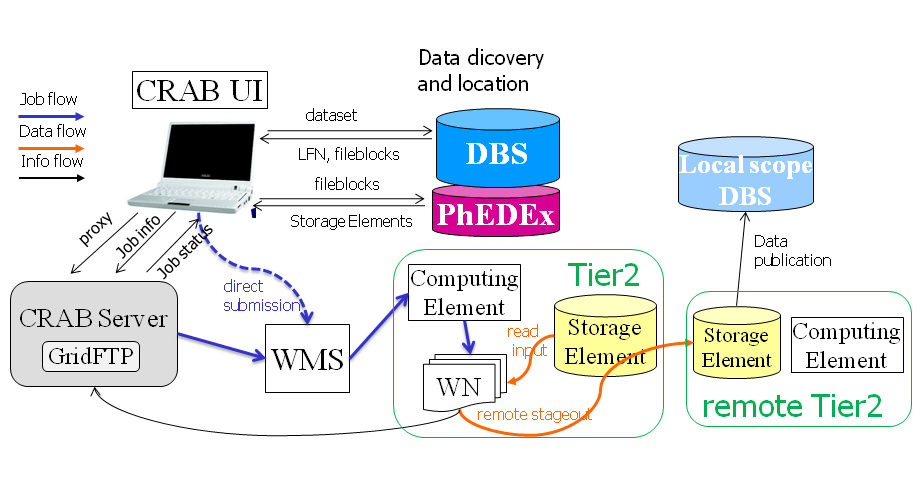
\includegraphics[width=0.70\textwidth]{figures/CRABWorkflow.png}
\caption{CRAB workflow. WMS can stand either for gLite WMS or glidein WMS.}
\label{fig:CRABWorkflow}
\end{figure}

\subsection{Job Monitoring}
\label{sec:3_3}
Monitoring tools are critical to the success of the
highly distributed analysis scenario in CMS.
%It was clear since the early days of CMS Analysis that
%good monitoring tools are critical to the success of such
%a highly distributed project.
Good monitoring has allowed CMS to evolve tool development
and operational structure from vision and anedoctal driven
to a fact based approach.
A few main points drove the development of monitoring tools:
\begin{itemize}
\item no reliance on local site monitoring.
\item a single  high level view of the usage from which
  to drill down to single job level
\item   keep the system lean and flexible: even if a few
  jobs are not properly reported
\item record
  enough information about failures so that plans and actions are set
  based on quantitative facts and that effectiveness of solutions can be metered
\item detect overall usage patterns to guide management into making
 choices and plans about how and were to steer user activities and
 how to plan for the future
\item do not try to define a priori all the relevant metrics
\end{itemize}

Job monitoring was built around the idea of instrumented
application: CMS jobs and tools send messages
to a central collector. Only jobs that use the
instrumented submission framework can be monitored in this way,
a small penalty in CMS case where almost
all user jobs are submitted using the CRAB tool.
The implementation is based on a
database running on Oracle server, a set of information collectors
feeding from various sources, 
and a few web interfaces (views) providing access with different levels
of detail, aggregation and flexibility, customized to
typical use cases, it is possible to cross link and navigate
from one view to another providing both extreme flexibility
and fast access to desired informations.
This set of tools is called ''the CMS Dashboard''.

\subsubsection{History View}
The aim here is to present time history of relevant
metrics to highlite overall patterns and trends.% (see Fig.~\ref{fig:HistoryView}).
%\begin{figure}
% 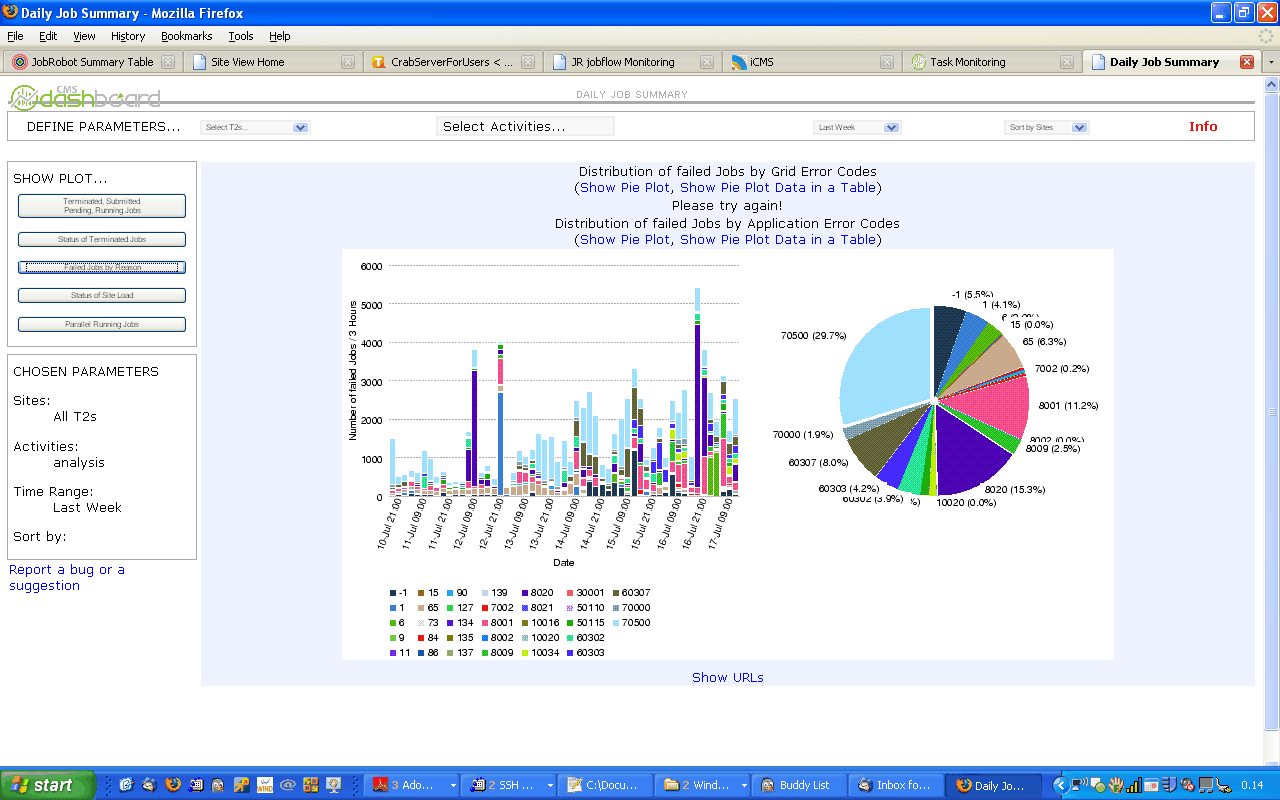
\includegraphics[width=0.70\textwidth]{figures/HistoryView.png}
%\caption{Dashboard History View}
%\label{fig:HistoryView}
%\end{figure}
The list of viewable metrics is predefined, and
the interface uses aggregated tables in the DB to provide
efficient access to old information with a limited
amount of detail. Data can be viewed divided
%according e.g. to the used site(s), job type or job completion status.
according to the used site(s) or job type or job completion status, among others.

\subsubsection{Task Monitoring for Analysis user}
A user centric view where the user is
initially presented the list of tasks he submitted in lasts
two days, both in tabular and graphical way (see Fig.~\ref{fig:TaskMonitor1}).

The user can then expand one selected task to get
a graphical overall summary of execution/completion progress
and access details of each job (see Fig.~\ref{fig:TaskMonitor2}).

\begin{figure}
\begin{minipage}{.45\textwidth}
\centering
 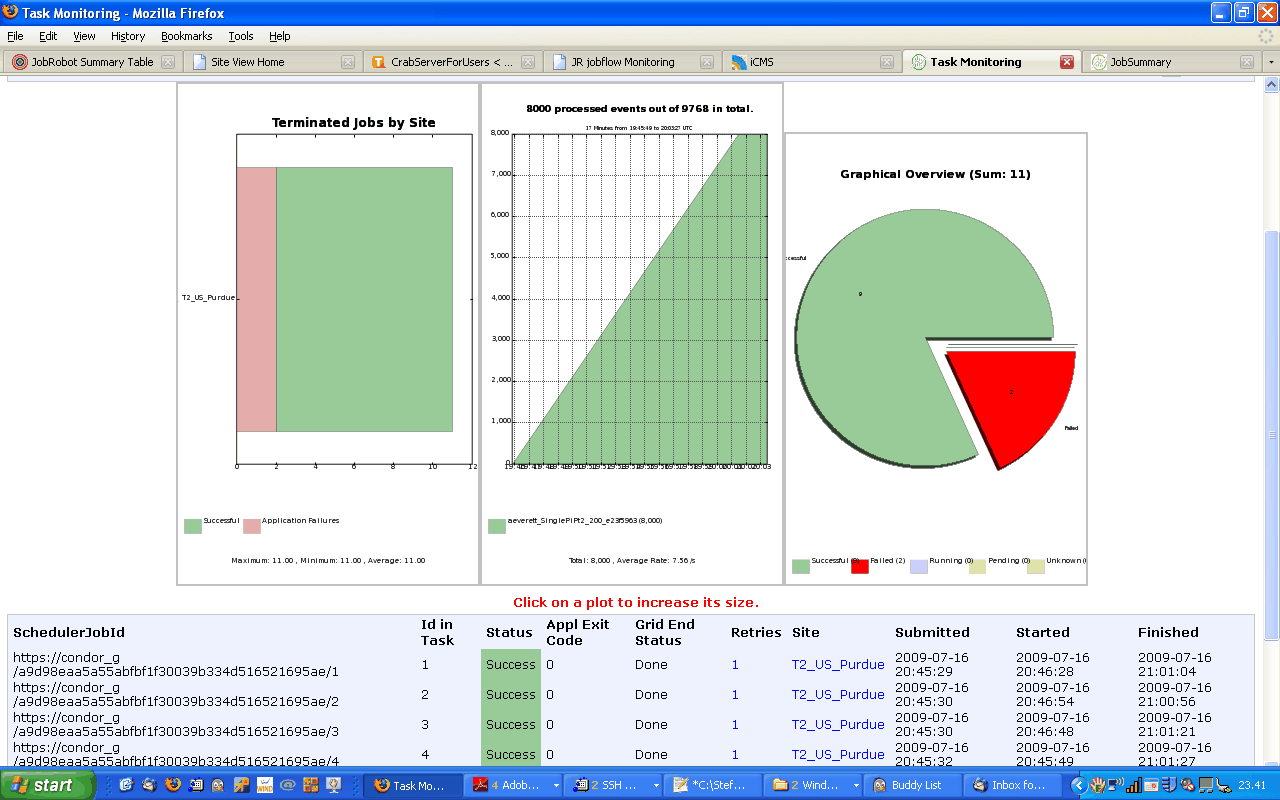
\includegraphics[width=0.95\textwidth]{figures/TaskMonitor1.png}
\caption{All users tasks in last 2 days}
\label{fig:TaskMonitor1}
%\end{figure}
%\begin{figure}
\end{minipage}
\begin{minipage}{.45\textwidth}
\centering
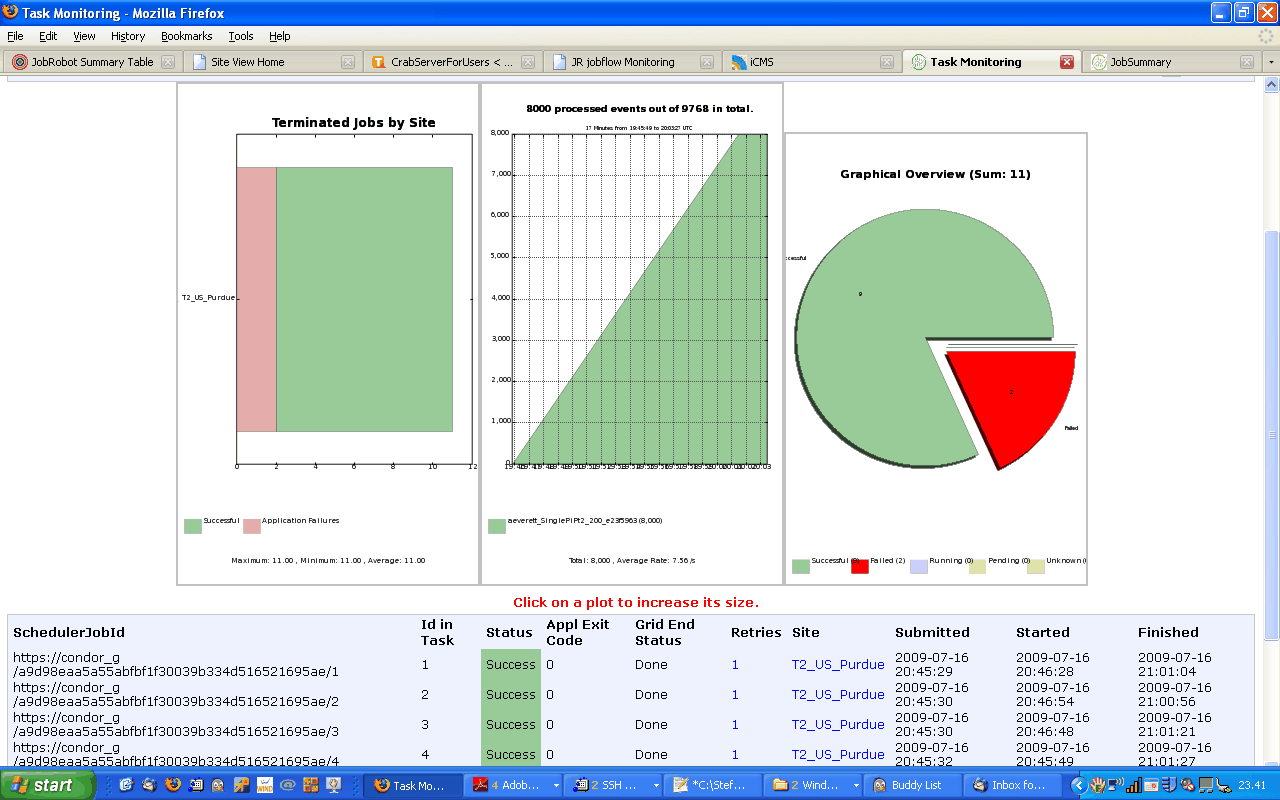
\includegraphics[width=0.95\textwidth]{figures/TaskMonitor2.png}
\caption{Expanded view of one task}
\label{fig:TaskMonitor2}
\end{minipage}
\end{figure}

\subsubsection{Interactive Interface}
Was the first view to be developed, based on
vision more then experience, therefore
emphasis was put on flexibility. It is a job-centric view
aimed at understanding and debugging what happens ``now''.
The entry point is the number of jobs submitted or
terminated in a chosen time period (see Fig.~\ref{fig:Dashboard}).
\begin{figure}
 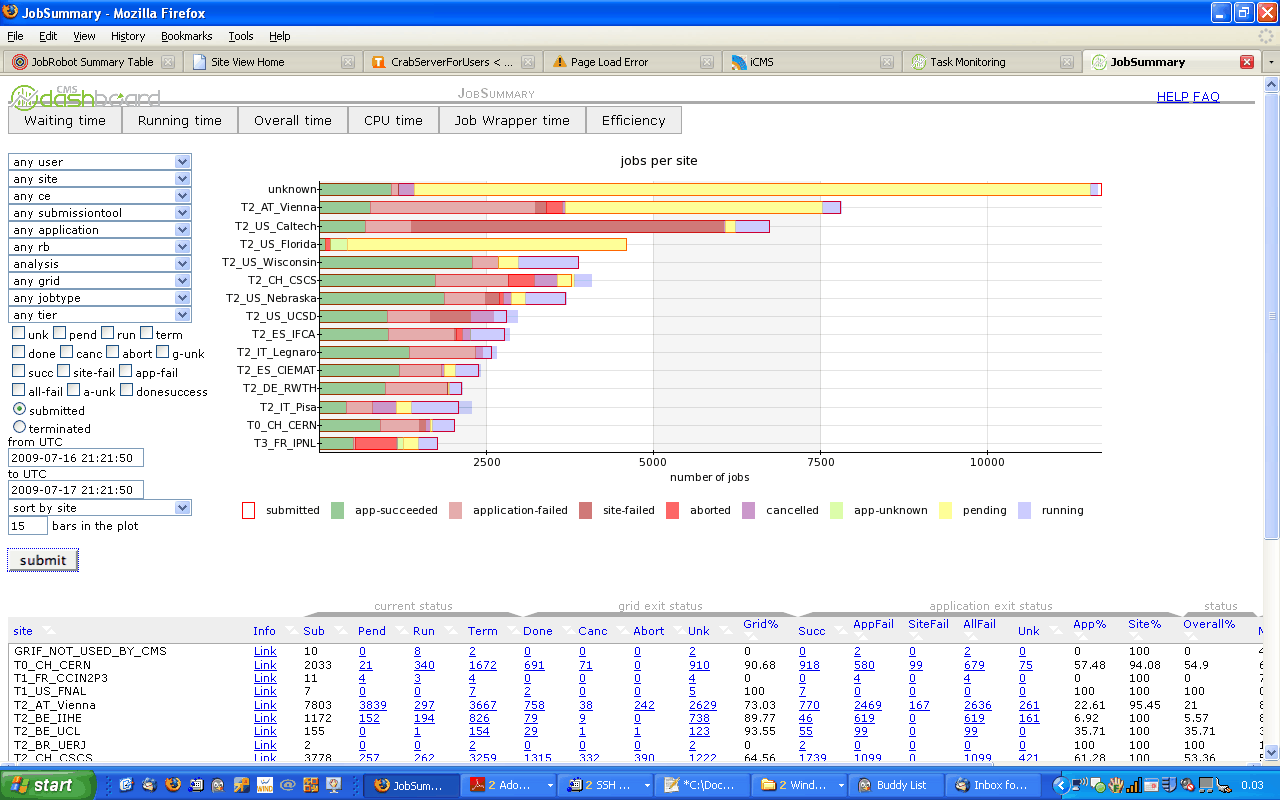
\includegraphics[width=0.80\textwidth]{figures/DashboardInteractive.png}
\caption{Dashboard Interactive Interface}
\label{fig:Dashboard}
\end{figure}
The interactive interface allows to drill down expanding the set of jobs by
various relevant properties (execution site, grid gateway,
submitter user, completions status, grid workload management host,
activity type, used dataset etc.), until all details stored in the DataBase
about a choosen (set of) job(s) can be accessed.
The interface reports success/failure
according to grid/site/application problem, and information
on used wall and cpu time of jobs.

\section{Operation of CMS Distributed Analysis}
\label{sec:4}
\subsection{Distributed Infrastructure}
\label{sec:4_1}
The tools described before operate on a distributed infrastructure
of sites offering uniform access via standard Grid services, moreover CMS maintains
sofware libraries at each site to get a uniform execution
environment. A small DataBase is used to keep track of
information specific to each site and relevant for CMS operations.

\subsubsection{ Grid services }
\label{sec:4_1_1}

The access to CMS resources is controlled by grid services provided by the WLCG project.
%Users are authenticated via X.509 certificated issued by trusted Certificate Authorities (CA).
Authorization is based on X.509 certificates extended with VOMS attributess
that certify the membership of users in the CMS Virtual Organization and possibly 
to CMS groups and the roles they have.
VOMS servers are provided by the WLCG project.
Data are stored on systems exposing an SRM interface (Storage Elements).
The specific implementation of the storage system is left to the sites
(e.g. d-Cache, DPM, Castor, Storm, etc...). In CMS Tier-1s the storage
systems also have a tape-based back-end to fulfil their custodial
responsibilities, while at Tier-2s they are disk-based.

The access to computing resources (Compute Elements) is based on
the Globus gatekeeper (on EGEE via its LCG-CE implementation) or on the ARC-CE on NorduGrid.
The CMS workload management system (CRAB and ProdAgent) may use, via the BossLite layer,
several high level workload management tools provided by the different infrastructures
(see~\ref{sec:CRAB}).


All computing and storage resources publish information on their
characteristics and state to an Information System based
on the BDII provided by WLCG. The information is used both
for monitoring and for resource selection.

The CMS data transfer system is implemented by PhEDEx that
in turn depends on the gLite File Transfer System (FTS).
WLCG maintains a number of FTS servers (at Tier-0 and Tier-1 sites)
that provide the transfer channels on which the transfers take place.
%Should you say here that FTS uses SRM which in turn uses gridFTP ?

%CMS established a body to coordinate the operation of the facilities offering support to the experiment. The Facilities Operations team coordinates the operations at all sites (Tier-0, Tier-1s and Tier-2s) in close collaboration with the site managers and with the WLCG project.

\subsubsection{ SiteDB }
\label{sec:4_1_2}
%% From DanieleB
SiteDB is a catalogue of all CMS computing Tiers.
It records the CMS resources at the site, the resources pledged for the future,
and it keeps track of CMS personnel at each site, including the roles
and duties they fulfill in the collaboration.
%Collaborators are automatically added to the SiteDB database on registering with the CMS Hypernews system. As well as providing the aforementioned information, SiteDB acts as a simple monitoring portal, bringing  in and providing links to content from PhEDEx, DBS, SAM tests, CMS Dashboard, GOCDB and GSTAT. The database also maintains a mapping between the different names a site can be known by, for instance the institute name (University of Bristol), its SAM/WLCG name (UKI-SOUTHGRID-BRIS-HEP), and the CMS name (T2_UK_SGrid_Bristol), as well as associations between sites (e.g. the parent T1 site for a T2)
CMS has designed and built SiteDB because CMS relies on close contact
to the sites it uses. The distributed nature of CMS computing makes
it very useful to track the people's responsbilities, and to contact
them on the basis of their role. Some site roles are technical
 (for instance running PhEDEx) others are related to CMS computing
 policy (e.g. the site's Data Manager).
%For users (both end users, and consumer of the info like the computing shifters) who have a problem with a site and may not know what the various roles and responsibilities are at a site, SiteDB provides this information. 
%In additions, SiteDB links to the CMS Savannah Computing Infrastructure portal, one of the tools CMS uses for internal  tracking of problems across the distributed infrastructure. In Savannah there is a group ('squad' in Savannah jargon) per site, dynamically maintained from the information in SiteDB via a set of cron-tabbed scripts.

\subsubsection{ Software Installation }
\label{sec:4_1_3}
%% Contributed by Ch.Wissing
%% Should be cross checked by Bockjoo
Distributed analysis relies on the experiment software being
pre-installed on the remote sites for each release. The CMS software
is packaged using the RedHat Package Manager (RPM), which is used by
some major Linux distributions. Dependencies between packages are
resolved with the help of the apt-get tool, which is also widely used in
the Linux community. The whole CMS software installation gets installed
on a filesystem shared among all worker nodes of a site.

During the
first setup of CMS software (``bootstrap'') the underlying operating system gets
checked for all required packages. These are imported into a meta-RPM,
which gets installed in the CMS software area. From that point on all
CMS installations are independent of the underlying operating
system. In addition to the actual CMS software (CMSSW) releases some ``external'' 
packages are installed, e.g. clients for databases, various ROOT
versions and GEANT4.

The installations itself are performed by high priority Grid
jobs. Those jobs are sent using a dedicated VOMS role %(lcgadmin) 
in order gain write access to the CMS software area. Once a release is
installed a tag is set on the %CE 
site that publishes the availability of
the release. The tags are used by the workload management systems to
submit jobs to sites that provide the requested CMS release.
Typically there about 10 production releases installed at a time at all
sites requiring roughly 50\,GB.

All software deployment and  removal activities are handled centrally
using two different instances, one for OSG based sites and one for
gLite and ARC based sites. Including Tier-1, Tier-2 and Tier-3
sites about 80 sites are served routinely.

\subsection{Infrastructure readiness}
\label{sec:4_2}
Operation of the CMS distributed infrastructure requires a stable and 
reliable behaviour of the services.
CMS has established a procedure routinely operated by the Facilities 
Operations team to extensively test all relevant aspects of sites 
supporting CMS~\cite{RefSite}, such as the ability to efficiently use their 
network to transfer data, the functionality of all the site services relevant 
for CMS and the capability to sustain the various CMS computing workflows at 
the required scale.
% AF is not sure how that steering occurs..it does not for the time being in analysis
%Result of the tests are combined in a "Readyness" metric that is used to 
%steer activity toward sites with higher Readyness mark.

\subsubsection{ Sites }
\label{sec:4_2_1} 
%\emph{USE THE COMMISSIONING PAPER AT CHEP09 CR2009-089}
%\emph{USE site commissioning section in INTEGRATION PAPER AT CHEP09 CR2009-087}
Every day the following quantities are monitored:
the CMS Service Availability Monitoring (SAM) tests to check sites basic 
functionality and local CMS software and configuration;
the success rate of the Job Robot, a load generator simulating
user data analysis; the number and the quality of the data
transfer links used in production by the site;
the downtimes scheduled by the site.
If any of the metrics based on the above information is not satisfied the site is declared in error state. A site is allowed to be in error state
not more than two days over the last week, then it is declared "not ready".
To recover from a "not ready state" the site needs to be ok for at least two consecutive days. In this way temporary glitches are allowed if recovered promptly.

\subsubsection{ Data transfer links }
\label{sec:LinkCommissioning}
%% From DanieleB & Nicolo'
A site needs to have sufficient data transfer connections to other sites in
order to perform CMS workflows. 
An ad-hoc task force (Debugging Data Transfers, DDT)\cite{RefDDT}
was created in 2007 to coordinate the debugging of data transfer links,
in order to commission most crucial transfer routes among CMS Tiers 
by designing and enforcing a clear procedure to debug problematic links.

A LoadTest infrastructure was set up in a separate debug environment of PhEDEx
to handle DDT test traffic.
The task force was charged with scheduling LoadTest transfers, assisting site
administrators with the configuration of data transfer middleware,
troubleshooting transfer issues, and documenting common problems and solutions.
The DDT procedures are now regularly used to certify links quality.

In order to pass commissioning criteria, a data link from Tier-0 or Tier-1s must
demonstrate a rate of at least 20 MB/s over 24 hours. Recognizing that uplinks
from Tier-2 to Tier-1 sites have a lower requirement in the computing model,
they are only required to transfer 5 MB/s. Links were routinely exercised and
were only decommissioned if they failed to meet these requirements for three
days in a row. Transfer quality on commissioned links is continuously monitored
with low rate transfers.

All Tier-0/1 to Tier-1 links are currently commissioned. 37 Tier-2 sites have
all of their downlinks from Tier-1 sites commissioned, and 2 more have seven out
of eight links commissioned. 47 Tier-2 sites have at least two commissioned
uplinks to Tier-1 sites.

\subsection{Analysis Organization at CMS Sites}
\label{sec:4_3}
\subsubsection{ Organized Analysis Activities }
\label{sec:4_3_1}
In order to optimize the processing chain, CMS performs as many processing
steps as possible in an organized way. 
Besides the re-processing %that is performed by the Data Operation team 
on the raw data when improved reconstruction algorithms are available,
a standard set of analysis passes is agreed with the physics groups
and is performed promptly at the Tier-1 sites 
%by the CMS Data Operations team 
as the data arrive from the Tier-0 (or Tier-2 in case of simulated data). 
This step, known as skimming, performs data reduction both
in terms of event size and number of events. 
The samples produced in this way are made available
to the CMS physicists at the Tier-2s. % together with the AOD.

Normally only the team dealing with data processing operations (Data Operation)
has access to the Tier-1 resources but in some special cases
some physicist may need access to large samples of raw data,
which can not be hosted at Tier-2's.
Examples of this kind of activity are the detector 
calibration or the Data Quality Monitor validation.
A special VOMS role has been created to grant access
to the Tier-1s to those physicists. 

\subsubsection{Physics groups and Users Activities}
\label{sec:4_3_2}
Physicists are organized in Physics groups each with its own internal 
organization.
Each Physics groups is associated with a few Tier-2 sites that support it by 
providing storage space and processing power.
Each Tier-2 supports one or more Physics groups depending on its size.
Currently, the association of Physics groups to sites is only reflected in policies for data location, but it is also foreseen to exploit VOMS groups to prioritize CPU usage at sites.

A nominal Tier-2 in 2008 had 200TB of disk-based storage.
Making efficient use of the overall space is a challenging data management exercise.
The current approach is decentralized administration with central oversight.
The knowledge of the needs is aggregated in the group leaders who will decide which data should be hosted at Tier-2 for their community. To help
them in the process, each Physics group is allocated a limited number 
of 'quanta', each being currently 30TB of disk and enough CPU to process it, hosted at few Tier-2s. 
%AF: I am not aware the following statment being true
%Central support advices PG leaders in selecting the specific location among the few available to each.

%\subsubsection{Users space}
Each Tier-2 site also supports a local community of users, providing them
a common space for data of local interest and a grid-enabled
storage for each user where to e.g. receive output from CRAB jobs
running at other sites. Each CMS user can access any data
hosted at any Tier-2, but can only write at the Tier-2 that supports him
as a local user.

The user produced data stored at a Tier2 can also be published into a local DBS
in order to allow their access to other collegues.
The data that is going to be accessed by many users or transferred among sites %are of more wide interest
, for instance the Physics Group specific event filtering and selections,
could be exposed to the entire collaboration by registering it in Global DBS and performing its transfer with PhEDEx.
User data is typically not produced with files large enough for wide area transfers or suitable for storage systems. Therefore a migration process involving the merge of the files and the validation of the data is foreseen before the registration in Global DBS and PhEDEx occurs.
 
\subsubsection{Storage hierarchy at Tier-2}
In order to support all the functionalities the CMS model requires the Tier-2 storage is divided into 4 logical pieces:
\begin{itemize}
\item{} Local Group and User Space: roughly 30TB for the local community and additional 1TB per user.
\item{} Physics Group Space: 60-90TB of space is allocated to serve 2-3 Physics Groups. Representatives from the groups serve as data managers for the space and make subscription and deletion requests.
The space for each group will increase with time as datasets grow.
\item{} Centrally Controlled Space: 30TB of space is identified at each Tier-2 under the control of CMS centrally.
This is used to ensure complete copies of the reconstruction datasets are available across the Tier-2s. This space can be further used as a flexible buffer to deal with operational issues and difficulties in the short term.
\item{} Simulation Staging and Temporary Space: 20TB is identified to
stage simulation produced at the Tier-2s and other temporary
files before they can be transferred to the permanent home. 
\end{itemize}

\subsection{User support model}
\label{sec:4_4}
User documentation is provided by a set of twiki pages composing the so called CMS Workbook. Documentation about the distributed environment and CRAB usage are available, as well as a troubleshouting guide.
Tutorials including hands-on session are periodically organized.
The day by day support is currently performed mainly via a mailing list (HyperNews) where users reports the problems they are facing. The reported problems range from problems with the infrastructure, 
site related issues to user's mistakes in tools configuration or real bug report that are feed back to developers.
The CMS Savannah Computing Infrastructure portal is used to report problems across the distributed infrastructure such as data access problems, problem on specific CMS software version at sites etc.

\section{Experience with CMS Distributed Analysis}
\label{sec:5}

Distributed Analysis has been ongoing for several years, passing through sequentially planned steps of 
increasing complexity, the so called data and physics challenges~\cite{RefPastExp}. 
It has been used extensively during studies to prepare the CMS Physics Technical Design Report~\cite{PTDR} and various detector commissioning activities. 
Last year experience both in term of dedicated commissioning tests and real users analysis is reported in the following sections.

\subsection{Analysis exercises within Common Computing Readiness Challenge}
\label{sec:5_1}
During the Common Computing Readiness Challenge (CCRC08) in May 2008
various analysis exercises were performed to gain an overall understanding 
of the performance and readiness of the Tier-2 sites for CMS data analysis.
Centrally organized job submissions were carried out both to understand the site performance characteristics and to exercise closely the kind of workflows
expected by the physics groups.
\paragraph{Site performance measurement}
Different types of jobs, with increasing complexity, were used:
\begin{itemize}
\item long-running CPU intensive jobs with moderate I/O. This tests the basic submission and execution of an analysis job with no strenuous requirements on 
either submit rate, or I/O, or stageout. The goal here was to fill all batch slots available for the analysis at a given site without stressing the site.
\item long-running I/O intensive jobs provided some non negligible stress on 
the storage infrastructure at the sites.
\item short-running jobs O(10 min) with local stage out of O(10 MB) file as output. These jobs run for a short time, with many jobs finishing per hour, thus leading to a significant write request rate at large sites.
\end{itemize}
Up to 40 sites were involved across EGEE, OSG, and NorduGrid. More than 100,000 jobs succeeded throughout the challenge. The error rates were very mixed, ranging from less than 1\% at many sites to up to 50\% at a few sites due to
catastrophic storage failures. The failures were predominantly
due to storage problems at sites. In most but not all cases, those problems were detected and fixed by the site administrators within 24 hours. Ignoring the storage failures, the success rate in this exercise was found to be better than 99\%. Overall success rate including the storage issues, ranged between 92-99\% for these exercises.

\paragraph{Simualtion of physics group workflows}
An exercise to mimic realistic physics group activities running
on a list of associated Tier2s was setup. 
%association of a list of T2s to each fake physics group
The CRAB server was used to submit realistic physics group tasks: 
analysis-like jobs reading a dataset at all sites and running for 
about 4 hours with remote stageout of a O(20 MB) output file to a subset of T2
sites. This simulates the computing model where each user has space at a T2 while the datasets are generally distributed throughout the world.
More than 100,000 jobs on about 30 sites were submitted in two weeks and 
the CRAB Server provided the needed functionality for job submission and 
tracking. %It is worth noting that the aim of this challenge was to test 
%the readiness of sites, by filling their resources, rather than a scale test of the CRAB Server.
Most failures were problems accessing the input data, from 0.1\%-10\% up to 50\% for pathological cases, and remote stageout issues were due to old Grid clients affecting from 100\% to few \% per site. These stageout issues were
promptly fixed by the site administrators. 
%Grid aborted jobswere usually reported via Global Grid User Support (GGUS)
%[] web with fast feedback from the sites. 
During the second week, sites with efficiency above 90\% significantly increased, as shown in Figure~\ref{fig:CCRC08SiteEff}.
%% mention the chaotic pahse?
\paragraph{Chaotic job submissions}
People from T2 sites were encouraged to submit jobs to other T2 sites, for mimicking a chaotic job submission pattern. This activity was clearly visible in the CMS Dashboard, showing lots of user activities at several sites. Figure~\ref{fig:CCRC08Chaotic} summarizes the number of active users per site, including Tier-1s, Tier-2s, Tier-3s and opportunistic usage. Around 60 sites participated in these tests.

The CCRC08 analysis challenge drove the level of activity and participation at Tier2s to an unprecedented scale in CMS.

\begin{figure}
\centering
\begin{minipage}{.45\textwidth}
\centering
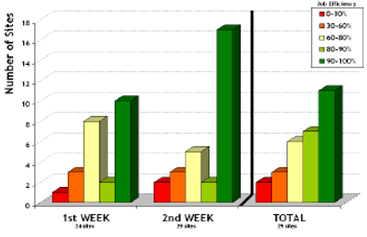
\includegraphics[width=0.95\textwidth]{figures/CCRC08SiteEff.png}
\caption{Distribution of the job efficiency by site, when simulating physics
groups workflows on CCRC’08}
\label{fig:CCRC08SiteEff}
%\end{figure}
%\begin{figure}
\end{minipage}
\begin{minipage}{.45\textwidth}
\centering
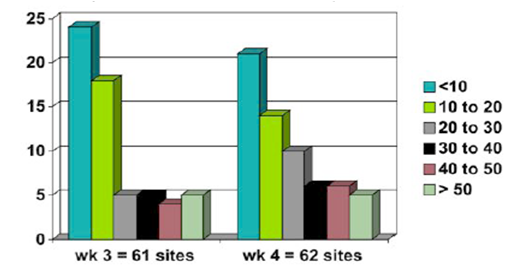
\includegraphics[width=1.\textwidth]{figures/CCRC08Chaotic.png}
\caption{Distribution of the number of users in a site, during the Chaotic phasein CCRC’08}
\label{fig:CCRC08Chaotic}
\end{minipage}
\end{figure}

\subsection{CRAB Analysis server stress test}
%% Scale test of CRAB server
%\paragraph{CRAB Analysis server stress test}
In order to test the CRAB Analysis server scalability and reliability up to
the expected CMS operational rates a dedicated test environment was
set up in October 2008. The Storage Element, based on GridFTP, 
that CRAB server relies on was installed on a different machine with 
respect to the machine hosting the CRAB Server components. The aim was 
to decouple the load
due the shipping of input/output sandboxes and the core workflow
management. The machine hosting the Storage Element and the CRAB
server were both 4 CPU 2000 MHz Dual Core AMD Opterons with 4 GB
RAM. The test was performed in the gLite context using two dedicated
gLite WMS. Monitoring information was collected from various sources
like the CRAB Server database tracking the job flow and the CPU usage
of its components, as well as from underlying services like MySQL and
GridFTP server and gLite WMS internal monitoring. The kind of
jobs submitted were very short jobs running for less than a few
minutes, not reading a dataset and without stage-out. This choice was
made to provide a harsher environment for job handling due to higher
rate of finished jobs and to limit the resource usage at sites.

%\begin{itemize}
%\item{   Single user phase}
%
%A single user performed a controlled job submission pattern: peaks of
%1000-2000 jobs every 5 hours superimposed on a constant rate of
%500-600 jobs every 20 minutes. Almost 200,000 jobs were submitted to
%more than 50 sites with a rate above 40,000 jobs/day, as shown in
%Figure \ref{fig:stresssingle}. The CRAB Server was able to cope with that
%rate with no indication of reaching a breaking point. No significant
%backlogs were accumulated. The main contributors to the load of the
%system were the MySQL and GridFTP usage, using about 2 and 1.5 CPUs
%\begin{figure}
%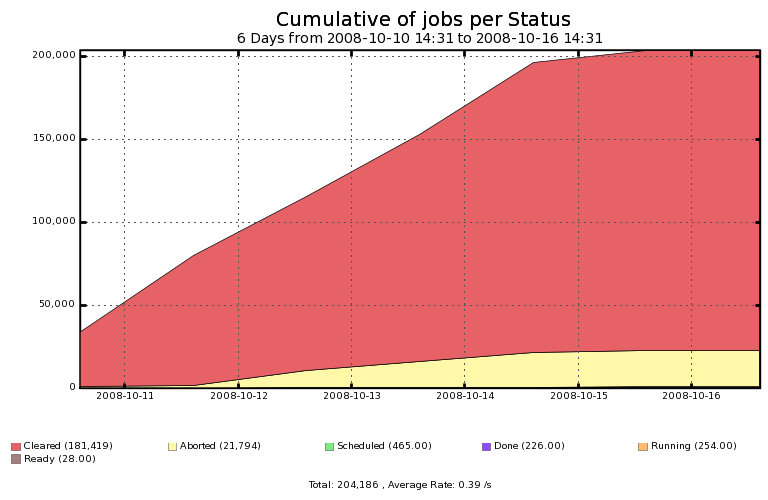
\includegraphics[width=0.55\textwidth]{figures/SingleUserJobStatus.png}
%\caption{Cumulative distribution of jobs submitted to CRAB Server
%  during the single user test phase. Aborted jobs were Grid related
%  problems at some sites. }
%\label{fig:stresssingle}
%\end{figure}
%
%\item{    Multi user environment phase}

Controlled submissions from different user certificates, thus 
emulating the CRAB Server usage in a multi-users environment, were performed.
%The need to further stress the multi-user environment arises
%from its higher complexity. Single threads of the very same component
%may be handling different user's jobs, requiring different
%certificates. Any interaction among them may cause failures, stopping
%the component work and causing a backlog.
Different submission patterns were adopted by the 12 users
involved. For example a user submitting 100 jobs every 15 minutes,
another 500 jobs every 20 minutes, another 2000 jobs every 6 hours
etc. plus a couple of users submitting randomly at their will.  No
CRAB Server misbehaviour was identified due to the multi-user
environment. %With respect to the single-user test 
Jobs were submitted to more than 50 sites with a rate above 50,000 jobs/day.
This helped identify some limitations in the communication between 
%JobTracking and GetOutput components 
the components responsible for job outpul retrieval and handling that caused a backlog of jobs without output retrieved. This effect is more evident for homogeneous very short
jobs, as those used in the test, that have a higher finishing rate
than real user's jobs which tend to finish at different times. None
the less, the backlog was absorbed in a few hours. This issue was
taken into account in the development cycle and the code was
optimized.  About 120,000 jobs were successfully handled in 48 hours,
as shown in Figure \ref{fig:stressmulti}.  The CPU load due to MySQL
proved to be stable regardless of the database size increase with more
jobs in the system. Overall the breakdown of CPU load usage is 2~CPUs
for MySQL, about 1.5~CPUs for GridFTP and about 1~CPU for all the CRAB
Server components, thus outlining the need of at least a 4~CPU
machine.  The load due to GridFTP is such that it's not compulsory to
have the GridFTP server decoupled from the machine hosting the CRAB
Server components.

The number of users currently using a CRAB Analysis Server is significantly 
increased with respect to the stress test scale, e.g. the growing number of real users using a CRAB Analysis Server instance over the last 5 months is shown in Fig.~\ref{fig:CSusers}.
Currently the whole CMS analysis is made of 30,000 jobs/day and the
CMS Computing model expectation is to reach around 100,000-200,000 jobs/day. 
Some CRAB Server instances deployed at different sites to serve physic's
group activities and regional community, as foreseen, can cope with
analysis needs.
%\end{itemize}
\begin{figure}
\begin{minipage}{.48\textwidth}
\centering
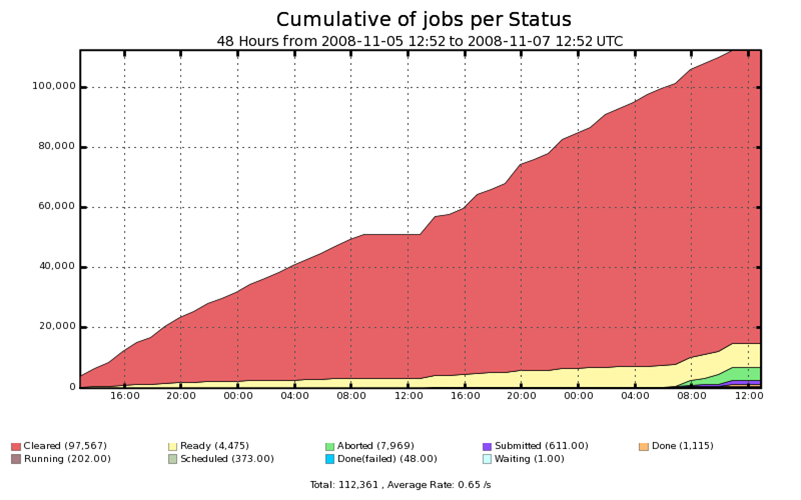
\includegraphics[width=0.99\textwidth]{figures/MultiUserJobStatus.png}
\caption{Cumulative distribution of jobs submitted to CRAB Server
  during the multi-user test phase. }
\label{fig:stressmulti}
\end{minipage}
\begin{minipage}{.48\textwidth}
\centering
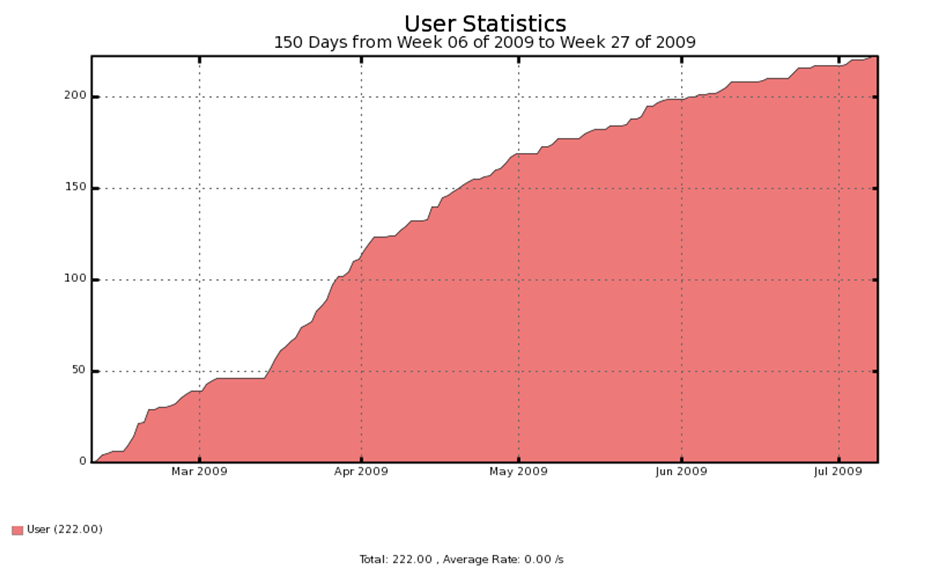
\includegraphics[width=0.99\textwidth]{figures/CSusersLast5months.png}
\caption{Number of distinct users using a CRAB server instance during last 5 months}
\label{fig:CSusers}
\end{minipage}
\end{figure}



\subsection{Sustained Analysis}
\label{sec:5_2}

%\emph{Look at metrics/content of PADA ASTF CHEP09 PAPER CR2009-088}
% CPU and wall clock time success rates are about 80% (from a 2 months observation) 
Distributed analysis is regularly performed by users for studies of the CMS physics discovery potential based on MC simulation and of the cosmic data collected in detector commissioning activities.
The number of users is increasing over time. For instance since 2008 the number of distinct CRAB users has continously grown to more than 1000, as shown in Figure~\ref{fig:intuser}. This indicates a very broad usage of CRAB since it represents roughly 30\% of the whole CMS community.
The day by day distribution of CRAB users is shown in Figure~\ref{fig:distusers}. An average of 95 different users per day use CRAB to submit their analysis 
jobs. 

\begin{figure}
\begin{minipage}{.48\textwidth}
\centering
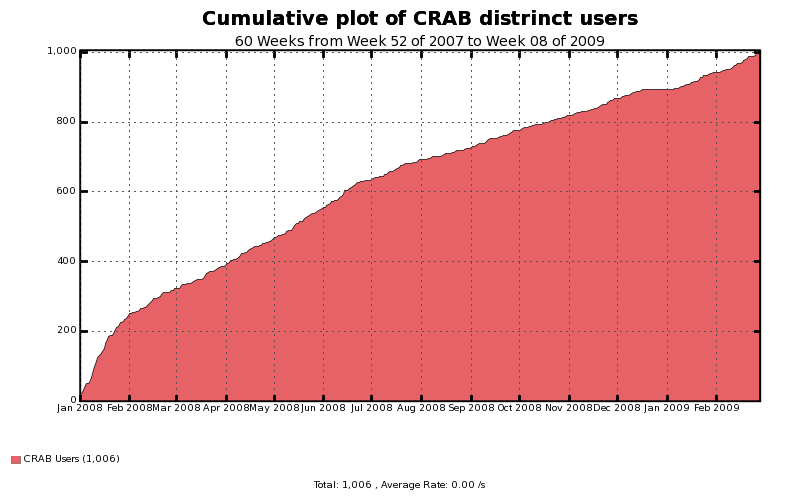
\includegraphics[width=0.99\textwidth]{figures/UserInteg.png}
\caption{Cumulative number of distinct CRAB users starting from 2008. }
\label{fig:intuser}
\end{minipage}
\begin{minipage}{.48\textwidth}
\centering
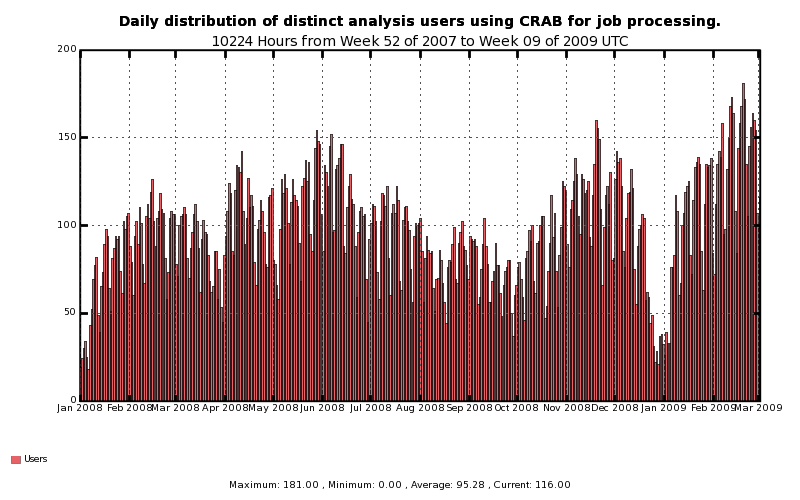
\includegraphics[width=1.2\textwidth]{figures/crabusersdaily.png}
\caption{Number of CRAB daily users in 2008. }
\label{fig:distusers}
\end{minipage}
\end{figure}


During last year about 11 million analysis jobs were submitted.  Peaks
of more than 100,000 jobs per day have been reached, with an average
of 30,000 jobs per day, as shown in Figure~\ref{fig:jobs}.
The distribution of analysis jobs at Tier-2s over the year is shown in Figure~\ref{fig:AnalysisJobHistoryApril0809}. Current analysis activities has spontaneously surpassed, both in term of number of jobs and number of sites, the scale reached in CCRC08 dedicated tests. 
\begin{figure}
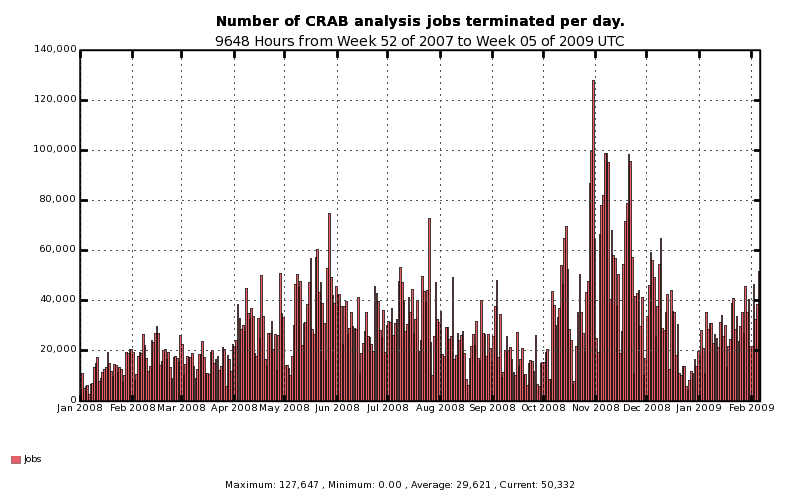
\includegraphics[width=3.5in]{figures/crabjobsdaily.png}
\caption{Number of daily jobs terminated in 2008. }
\label{fig:jobs}
\end{figure}

%Analysis job efficiency is summaried in Fig.~\ref{fig:AnalysisJobEffMay08March09}. 
The distribution of analysis job efficiency over time is shown in Fig.~\ref{fig:T2EffApril0809}. The average success rate is 61\% with 4\% of cancelled jobs, 10\% of grid failures and 25\% application failures.
Most of the failures faced by the users are due to remote stageout issues, user application errors and errors reading data at the site. 
Part of the failures are somehow expected, since analysis jobs run user code which may not have been thoroughly tested. For instance memory leaks or crash in rare events might be hard to spot in the small scale test typically done by the users.

Failures in stage out of the data output files to remote storage can be due 
to users misconfiguring the remote destination to use or to transfer problems.
A hanging or failing stage out represents a waste of CPU since it occurs at 
the end of the job processing, so an approach to decouple the job processing and the remote stage out is under development. At job finishing the output will be stored locally at the site and the remote stage out will occur in an asynchronous step.

Failures accessing data at the site mainly expose problems with the storage at the site or inconsistencies between the data catalogue and what has been deleted at the site. 
Periodically data consistency and integrity checks at all Tier-2 sites are performed. This check verifies that the contents of the disks at the Tier-2 sites are consistent with the PhEDEx databases and DBS and reduce the rate of data access errors.

Grid failures are due to underlying grid system but also reflect site problems or jobs that spend too much time on the worker node and are killed by the local batch system, appearing as aborted by the Grid.


% From April08 to April09:
% overall T2 analysis job efficiency 61%
% breakdown of failures:
% - Cancelled 4%
% - Grid failures 10% Aborted
% - Application errors 25%
%   40% remote stageout    ==> overall 10%
%   13% CMSSW error (8001) ==> overall 3%
%    6% error reading files at site (8020) ==> overall 1.5% 
%    9% cmsRun did not produce a valid job report (50115): Bad crash usually
%    2% error 1
%    2% problem with ModifyJobRepor (70500)
%    2.5% Config File Read Error (7002)
%
% From Jan09 to May09:
% overall analysis job efficiency 62%
% breakdown of failures:
% - Grid failures: 8% Aborted
% - Application errors:
%   35% remote stageout
%   22% CMSSW error (8001 , 8009) --> I suspect that some of the 8001
%                                      are due to error reading input files
%   13% error reading files at site (8020)
%    6.8% error 50115
%
\begin{figure}
\begin{minipage}{.55\textwidth}
\centering
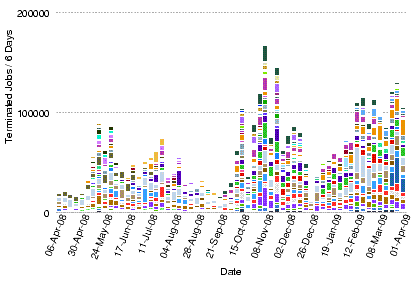
\includegraphics[width=1.0\textwidth]{figures/AnalysisJobHistoryApril0809.png}
\caption{Number of analysis jobs by Tier2s during last year from CMS dashboard History view. Each color refers to a site. }
\label{fig:AnalysisJobHistoryApril0809}
\end{minipage}
\begin{minipage}{.45\textwidth}
\centering
%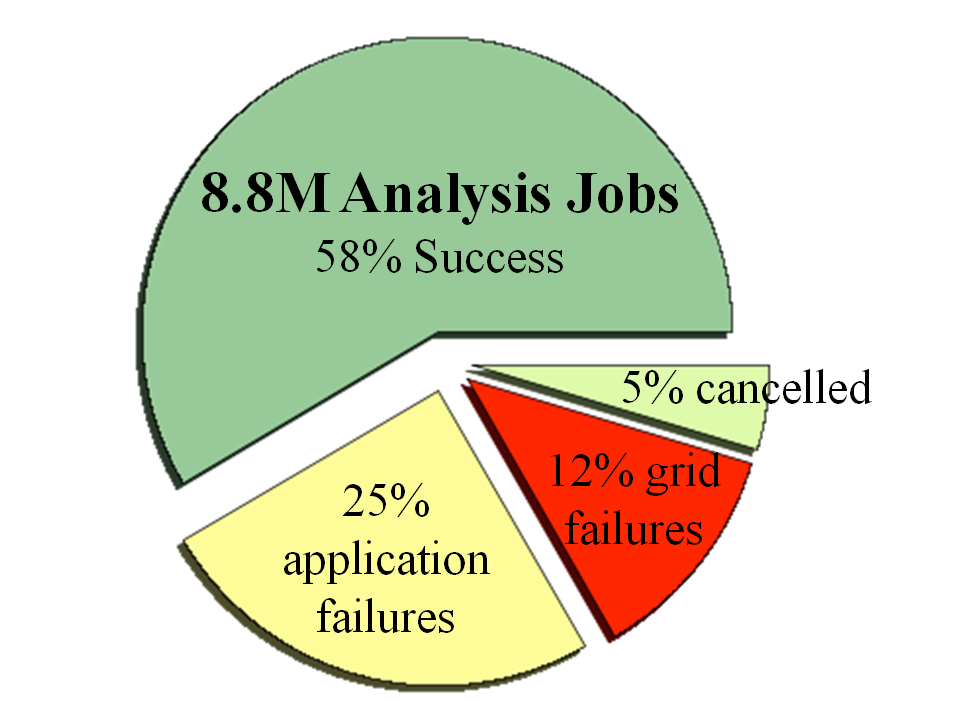
\includegraphics[width=0.5\textwidth]{figures/AnalysisJobEffMay08March09.png}
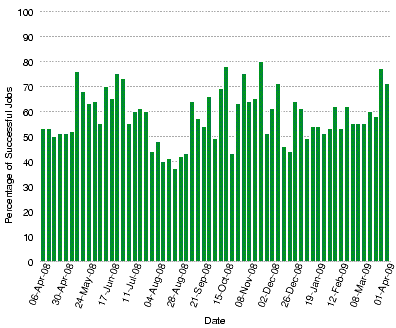
\includegraphics[width=0.9\textwidth]{figures/T2EffApril0809.png}
\caption{Analysis job efficiency during last year. }
\label{fig:T2EffApril0809}
\end{minipage}
\end{figure}

About 78\% of the CMS analysis jobs were submitted using gLite WMS.  Since the gLite architecture is such that the system scales linearly with the number of gLite WMSs used, analysis jobs are balanced currently over 7 WMS. The rest of the analysis jobs are submitted using Condor-G.

CRAB Analysis Server instances have been deployed in several countries (CERN, Italy, France). A couple of them are open to worldwide distributed CMS users. Other instances are being used by local communities or specific physics group.
%% CrabServer usage
% 33% of jobs in last 5 months submitted with Server (1.5M jobs), direct (3Mjobs) 
%The growing number of users using a CRAB Analysis Server intance over the last 5 months is shown in Fig.~\ref{fig:CSusers}.

A complete example of analysis activity during the year has been the analysis 
of real cosmic data collected during a long period of data-taking, called CRAFT (Cosmics Run At Four Tesla) to commission the detector in preparation for LHC collision. About 300 million events of cosmic muons were taken and their analysis is meant to assess detector perfomance and perfom physics studies.
% such as measurement of cosmic muon charge ratio or absolute cosmic muon flux as function of the muon momentum
The raw data were transferred at Tier-1 where several re-processing and data skimming took place. The reconstructed data were all shipped to the CAF where calibration and alignment studies were performed in order to provide better conditions to be used in subsequent re-processing. 
%All data at CAF: 122 TB
Reconstructed data and their skims were also spread to Tier-2s, manily to 
those associated with Muon and Tracker group although overall about 20 sites hosted CRAFT data. The overall amount of CRAFT data transferred at Tier-2s was more than 300TB.
%Total data of CRAFT data transfers at other T2s (19 sites):  ~315TB
The number of users analysing CRAFT data during the year is shown in Fig.~\ref{fig:CRAFTusers} where the breakdown of users using the CAF and those using the Tier2s is also reported. The distribution of analysis jobs is shown in Fig.~\ref{fig:CRAFTjobs}, roughly two third at Tier-2s and one third at CAF.
The job efficiency at Tier-2s is lower than that at CAF because, on top of the application errors, there are grid failures and the stage out error mentioned above.
%Effort in improving the success rate and regularly identifying problem areas are ongoing.
%=== at CAF: success rate 83% with 17% of application failures 
% application failures 37% CMSSW error,26% errror 50115 likely bad crash , 10% failures reading input files
% overall 6% CMSSW error, 4% bad crash , 2% input files 
%=== on Grid: success rate 48% with 35% of application failures and 17% of Grid failures 
% application failures :57% stageout, 18% CMSSW error, 7% reading input files)
% overall 20% stageout, 6% CMSSW error, 2.5% input files
%
\begin{figure}
\begin{minipage}{.48\textwidth}
\centering
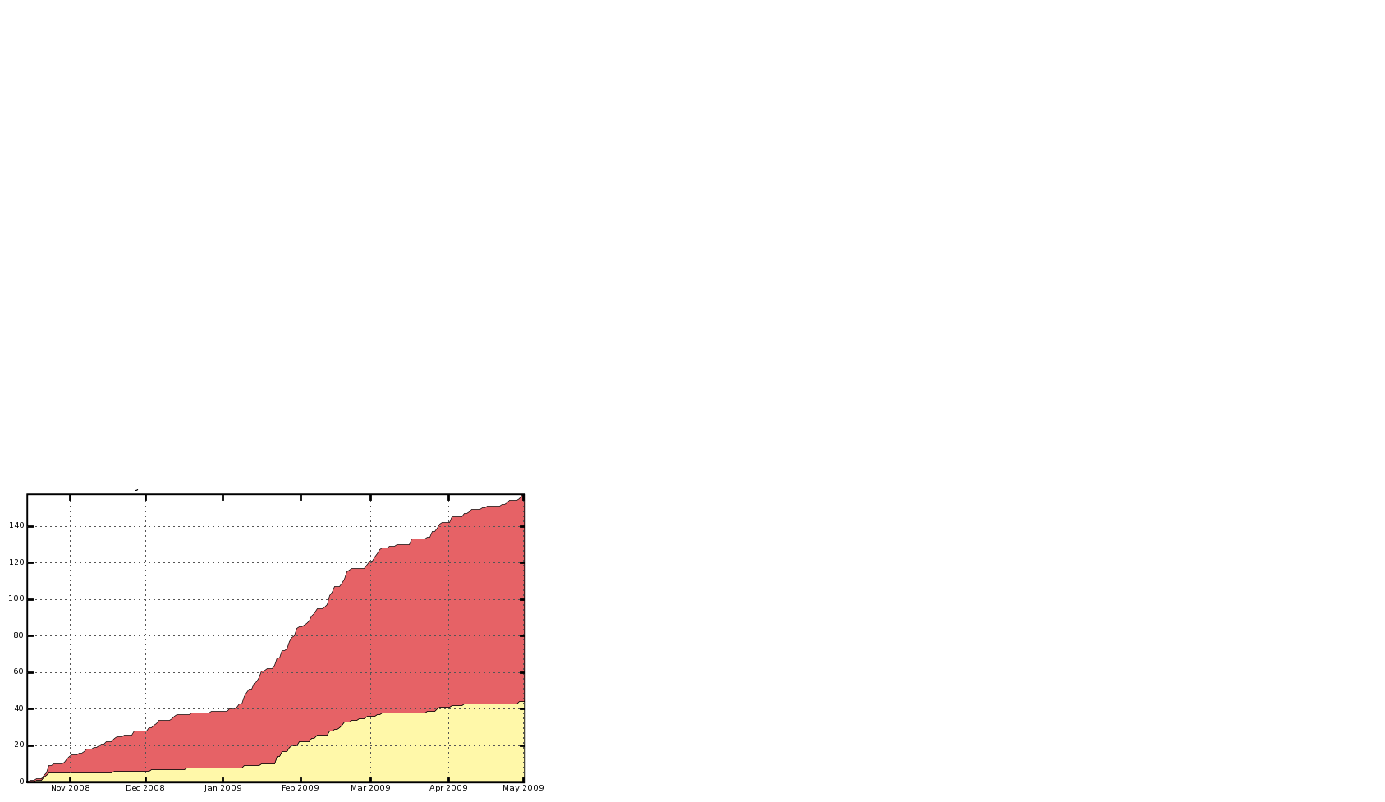
\includegraphics[width=0.94\textwidth]{figures/CRAFTusers.pdf}
\caption{Number of users analyzing CRAFT data using the CAF (light gray) or the Tier2s (dark gray).}
\label{fig:CRAFTusers}
%\end{figure}
%\begin{figure}
\end{minipage}
\begin{minipage}{.48\textwidth}
\centering
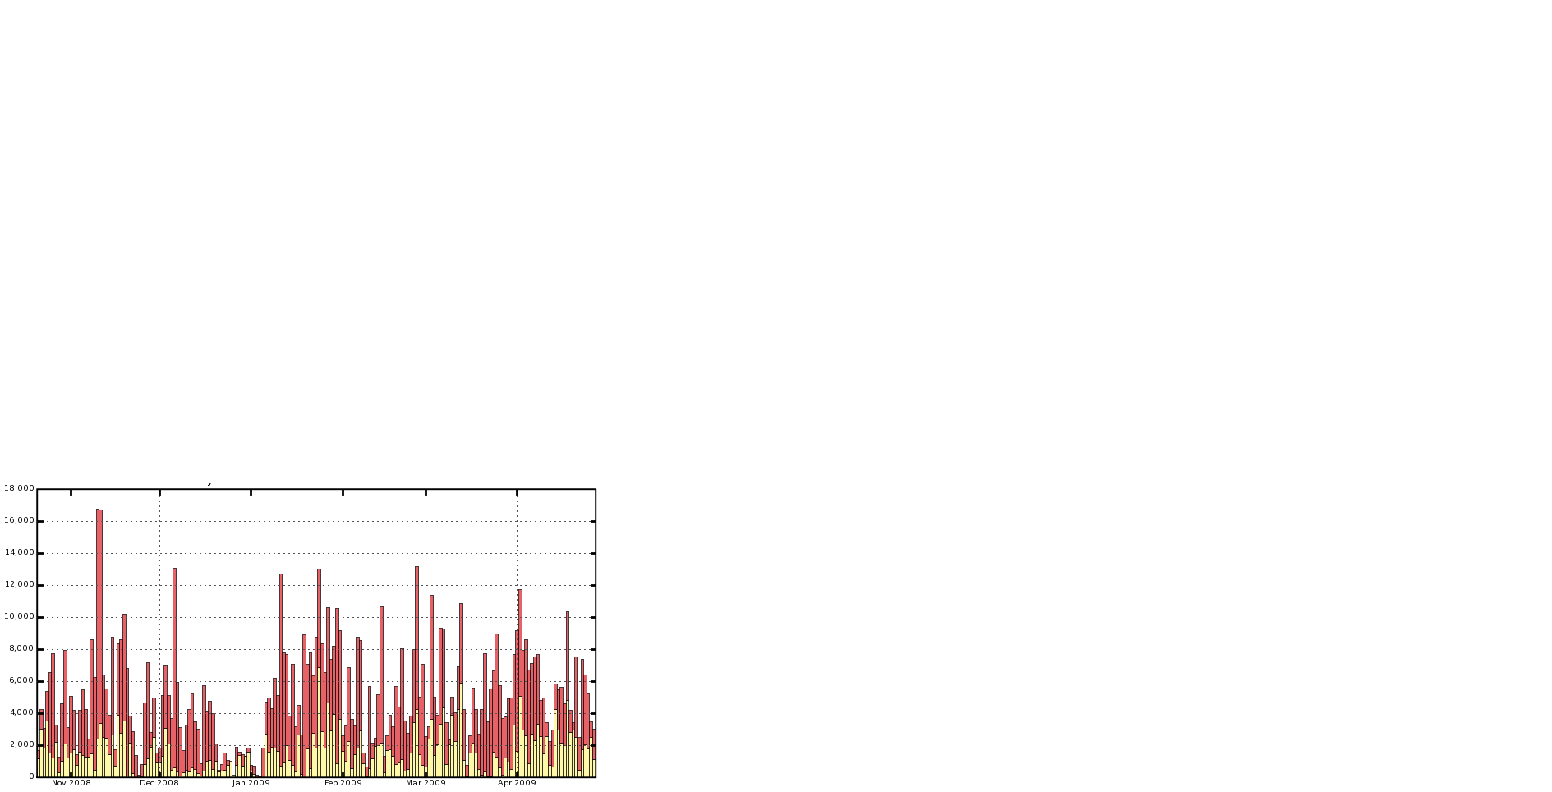
\includegraphics[width=1.06\textwidth]{figures/CRAFTjobs.pdf}
\caption{Number of jobs analyzing CRAFT data using the CAF (light gray) or the Tier2s (dark grey).}
\label{fig:CRAFTjobs}
\end{minipage}
\end{figure}


Real user analysis jobs show worse job efficiency (around 60\%) with respect to the efficiencies obtained during dedicated and controlled submissions such 
as computing challenge and Job Robot activities, described in ~\ref{sec:5_1} and ~\ref{sec:4_2_1} respectivelly.
Analysis specific operations to improve the success rate and user experience when utilizing the distributed computing environment and to ensure a functional system with a more efficient use of CMS resources on sustained user activities are being setup.

\section{Conclusions}
\label{sec:6}
Commissioning a distributed analysis system of the scale required by CMS
in terms of distribution and number of expected users is a unique challenge.
In order to prepare for large scale physics analysis CMS has established a set 
of operations to extensively test all relevant aspects of the distributed
infrastructure to support CMS workflows, such as performance and readiness of sites and transfer links.
The Workload Management and Data Management components of the Computing Model
are now well established and are constantly being exercised and improved
through CMS-wide computing challenges, and first real cosmic data taking
exercises, in preparation for the LHC collision data taking.

\section{Acknowledgements}
We thank the technical and administrative staff of CERN and CMS Institutes,
Tier-1 and Tier-2 centres and acknowledge their support.

% For one-column wide figures use
%\begin{figure}
%% Use the relevant command to insert your figure file.
%% For example, with the graphicx package use
%  \includegraphics{cations, both on the client-side and on the
%% figure caption is below the figure
%\caption{Please write your figure caption here}
%\label{fig:1}       % Give a unique label
%\end{figure}
%


%% For tables use
%\begin{table}
% table caption is above the table
%\caption{Please write your table caption here}
%\label{tab:1}       % Give a unique label
% For LaTeX tables use
%\begin{tabular}{lll}
%\hline\noalign{\smallskip}
%first & second & third  \\
%\noalign{\smallskip}\hline\noalign{\smallskip}
%number & number & number \\
%number & number & number \\
%\noalign{\smallskip}\hline
%\end{tabular}
%\end{table}

%\begin{acknowledgements}
%If you'd like to thank anyone, place your comments here
%and remove the percent signs.
%\end{acknowledgements}

% BibTeX users please use one of
%\bibliographystyle{spbasic}      % basic style, author-year citations
%\bibliographystyle{spmpsci}      % mathematics and physical sciences
%\bibliographystyle{spphys}       % APS-like style for physics
%\bibliography{}   % name your BibTeX data base

% Non-BibTeX users please use
\begin{thebibliography}{}
%
% and use \bibitem to create references. Consult the Instructions
% for authors for reference list style.
%
% Format for Journal Reference
\bibitem{RefCMS}
CMS Collaboration R. Adolphi et al., The CMS experiment at the CERN LHC, JINST, 0803, S08004 (2008)
%
\bibitem{RefCM}
C.Grandi, D.Stickland, L.Taylor et al., The CMS Computing Model, CERN-LHCC-2004-
035/G-083 (2004)
%
\bibitem{RefDBS}
A. Afaq et al., The CMS dataset bookkeeping service, J.Phys.Conf.Ser, 119, 072001 (2008)
%
\bibitem{RefFrontier}
B. Blumenfeld,D. Dykstra,L. Lueking,E. Wicklund, CMS conditions data access usingFroNTier, J.Phys.Conf.Ser, 119, 072007 (2008)
%
\bibitem{RefPhEDEx}
R. Egeland et al., Data transfer infrastructure for CMS data taking, Proceedings of Science, PoS(ACAT08)033 (2008)\\
L. Tuura et al., Scaling CMS data transfer system for LHC start-up, J.Phys.Conf.Ser, 119, 072030 (2008)
%
\bibitem{RefPA}
D. Evans et al., The CMS Monte Carlo production system: Development and design, Nucl.Phys.Proc.Suppl.177-178, 285-286 (2008)
%
\bibitem{RefCRAB}
D. Spiga et al., The CMS Remote Analysis Builder CRAB, 14th Int. Conf. on High Performance Computing ISBN/ISSN: 978-3-540-77219-4 , 4873, 580-586 (2007)
%
\bibitem{RefWLCG}
LCG Computing Grid Technical Design Report, LCG-TDR-001 CERN/LHCC 2005-024 (2005)
%
\bibitem{RefBOSSLite}
G. Codispoti et al., Use of the gLite-WMS in CMS for production and analysis, Proceedings of International Conference On Computing In High Energy Physics And Nuclear Physics (2009). 
%
\bibitem{RefgLiteWMS} P. Andreetto et al., The gLite Workload Management System, J.Phys.Conf.Ser, 119, 062007 (2008)
%
\bibitem{RefOSG} R. Pordes et al, The Open Science Grid, J.Phys.Conf.Ser, 78, 012057 (2007)
%
\bibitem{Refglidein} I. Sfiligoi et al., glideinWMS - A generic pilot-based Workload Management System, J.Phys.Conf.Ser., 119, 062044 (2008)
%
\bibitem{RefARC} M.Ellertet al., Advanced Resource Connector middleware
  for lightweight computational Grids, Future Generation Computer Systems, 23, 219-240 (2007)
%
\bibitem{RefSite}
J.Flix, A. Sciab\`a et al., The commissioning of CMS computing centres in the worldwide LHC computing Grid, Conference Record N29-5 session Grid Computing, Nuclear Science Symposium IEEE , Dresden (2008)
%J.Flix et al., The commissioning of CMS sites: improving the site reliability, 
%Proceedings of International Conference On Computing In High Energy Physics And Nuclear Physics (2009). \emph{IS IT POSSIBLE TO REFERNCE NOT YET PUBLISHED CHEP09 PAPER?}\\ 
%\emph{IS THE ACAT REFERENCE READY?}

%
\bibitem{RefDDT} N. Magini et al., The CMS Data Transfer Test Environment in Preparation for LHC Data Taking, Conference Record N67-2 session Applied Computing Techniques, Nuclear Science Symposium IEEE , Dresden (2008)
%
\bibitem{PTDR} G.L. Bayatian et al., CMS Technical Design Report volume II: physics performance, Journal of Physics G: Nuclear and Particle Physics., 34, 995-1579 (2007)
%
\bibitem{RefPastExp} 
CMS collaboration,  CMS Computing, Software and Analysis Challenge in 2006 (CSA06) Summary , %CMS NOTE-2007/006 
CERN/LHCC 2007-010 (2007) \\
N.DeFilippis et al., The CMS analysis chain in a distributed environment, Nucl.Instrum.Meth. A559, 38-42 (2006) \\
A.Fanfani et al.,Distributed computing Grid experiences in CMS, IEEE Trans.Nucl.Sci.52,884-890 (2005)
%% Format for books
%\bibitem{RefB}
%Author, Book title, page numbers. Publisher, place (year)
\end{thebibliography}

\end{document}
% end of file template.tex

